\documentclass[border=10pt]{standalone}
\usepackage{tikz}
\usetikzlibrary{shapes.geometric, calc}



\begin{document}

  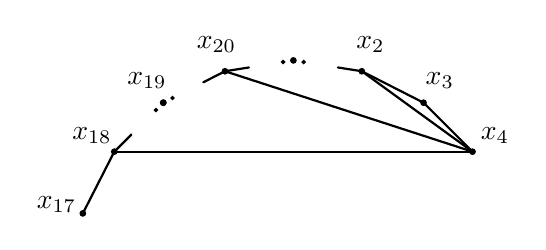
\begin{tikzpicture}[line cap=round]
	    \def\r{80pt} %radius of circumscribed circle
        \def\rn{90pt} %radius of "invincible" circle with edges numbered 

		  \pgfmathtruncatemacro\a{20} % number of polygon vertices



%%% full grid of rectangle with numbers

%\foreach \i in {1,2, ..., \a} {
%    \coordinate (p\i) at ({-\r*cos(\i*(360/\a) + (90-360/\a)},{\r*sin(\i*(360/\a) + (90-360/\a))});
%    \draw[fill=black] (p\i) circle (1pt); 
%              
%\node at (
%   {-\rn*cos(\i*(360/\a) + (90-360/\a)},
%   {+\rn*sin(\i*(360/\a) + (90-360/\a))}
%){\i};
%}		  

% select wanted edges by changed the first line of the code block below
\foreach \i in {2,3,4,17,18,19,20} {
    \coordinate (p\i) at ({-\r*cos(\i*(360/\a) + (90-360/\a)},{\r*sin(\i*(360/\a) + (90-360/\a))});
    \draw[fill=black] (p\i) circle (1pt); 
    
%comment code below and to hide numbers
\node at (
   {-\rn*cos(\i*(360/\a) + (90-360/\a)},
   {+\rn*sin(\i*(360/\a) + (90-360/\a))}
){$x_{\i}$};

}	

% draw complete paths
	
\draw[thick,black] (p2) -- (p3);
\draw[thick,black] (p2) -- (p4);
\draw[thick,black] (p4) -- (p20);
\draw[thick,black] (p3) -- (p4);	
\draw[thick,black] (p4) -- (p18);			
\draw[thick,black] (p17) -- (p18);		

% draw nodes between 2 other nodes (no numbers)
\foreach \i in {1,19} {
    \coordinate (p\i) at ({-\r*cos(\i*(360/\a) + (90-360/\a)},{\r*sin(\i*(360/\a) + (90-360/\a))});
    \draw[fill=black] (p\i) circle (1pt); 
    
%un-comment code below and to show numbers
%\node at (
%   {-\rn*cos(\i*(360/\a) + (90-360/\a)},
%   {+\rn*sin(\i*(360/\a) + (90-360/\a))}
%){$x_{\i}$}; %can also use {\i}
}

%draw halfway paths to depict generality	


\draw[thick,black] (p2) -- ($(p2)!0.35!(p1)$);
\draw[thick,black] (p20) -- ($(p20)!0.35!(p1)$);
%
\draw[thick,black] (p20) -- ($(p19)!0.65!(p20)$);
\draw[thick,black] (p18) -- ($(p19)!0.65!(p18)$);

\coordinate (etc1) at ($(p2)!0.5!(p20) + (0,0.1)$);

% draw neighbouring circles to node p1 to signal etc

 \draw[fill=black]  ($(p2)!0.85!(p1)$) circle (0.6pt);
 \draw[fill=black] ($(p20)!0.85!(p1)$)  circle (0.6pt);

% draw neighbouring circles to node p1 9to signal etc

\node at (p19) {.};
 \draw[fill=black] ($(p20)!0.85!(p19)$) circle (0.6pt);
 \draw[fill=black] ($(p18)!0.85!(p19)$) circle (0.6pt);


 \end{tikzpicture}
% 
\end{document}


